\documentclass[12pt]{scrartcl}

\usepackage{fontspec}
\usepackage{polyglossia}
\setdefaultlanguage{russian}
\newcommand{\docfont}{Times New Roman}
\setmainfont[Ligatures=TeX]{\docfont}
\newfontfamily\cyrillicfont[Ligatures=TeX]{\docfont}
\newfontfamily\cyrillicfontsf[Ligatures=TeX]{\docfont}
\newfontfamily\cyrillicfonttt[Ligatures=TeX]{\docfont}

\usepackage{amsmath,amsfonts,amsthm,amssymb} % nice math symbols
\newtheorem{definition}{Определение}
\usepackage{hyperref}

\hypersetup{%
	pdfencoding=auto,
	pdfauthor={Александр Панов},
	pdftitle={Операции в знаковой картине мира}
}
\usepackage{csquotes}
\usepackage{graphicx}
\graphicspath{{../../images/}}

\usepackage[plain]{algorithm}
\usepackage[noend]{algpseudocode}
\renewcommand{\algorithmiccomment}[1]{{\quad\footnotesize // #1}}
\renewcommand{\algorithmicrequire}{\textbf{Input:}}
\renewcommand{\algorithmicensure}{\textbf{Output:}}

\usepackage[
%	autolang=hyphen,
	language=auto,
	autolang=other,
	backend=biber,
	style=gost-numeric
]{biblatex}
\addbibresource{../../biblio/library.bib}
\DeclareSourcemap{
	\maps[datatype=bibtex, overwrite]{
		\map{
			\step[fieldset=langid, fieldvalue=english]
			\step[fieldset=doi, null]
			\step[fieldset=issn, null]
			\step[fieldset=isbn, null]
			\step[fieldset=url, null]
			\step[fieldsource=language, fieldset=langid, origfieldval]
		}
	}
}

\linespread{2}

\title{Структура знака и операции в знаковой картине мира}
\author{Г.\,С.~Осипов, А.\,И.~Панов\\
	{\large\slshape ФИЦ ИУ РАН, пр. 60-летия Октября, 9, gos@isa.ru}}

\begin{document}
%	\affil{ФИЦ ИУ РАН}
	
	\maketitle{}
	\begin{abstract}
		В работе представлен новый подход к интеграции знаний субъекта деятельности о внешней среде и своих характеристиках с операциями на основе этих знаний - знаковая картина мира. Основным элементом картины мира является четырехкомпонентная структура - знак, существование и строение которого подтверждается как психологическими теориями, так и нейрофизиологическими данными. В работе вводится специальная математическая структура - каузальная матрица, с помощью которой описывается строение компонент знака. Предложены процедуры пополнения отношений на множестве знаков, определены операции в знаковой картине мира, которые моделируют важные психологические особенности поведения человека.
		\par\bigskip
		\textit{Ключевые слова}: знаковая картина мира, образ, значение, личностный смысл, каузальная матрица, семиотическая сеть, обобщение.
	\end{abstract}
	
	
	\section*{Введение}
	Про постановку задачи \cite{Osipov2014c,Osipov2015d}.
	
	Психологические и нейрофизиологические основания трехкомпонентной структуры знака (Станович, Гроссберг и др. более новые).
	
	\section{Картина мира}

	Неформально про компоненты знака, функции связывания и три типа картин мира. Картина мира - это не только представление знаний, но и процедуры и операции, выполняемые на основе этого представления.
	
	\section{Строение компонент знака}
	
	Рассмотрим структуру компонент знака на примере образной компоненты, которая участвует в распознавании представляемого объекта или процесса на основе поступающей из внешней среды сенсорной информации и регистрируемой внутренними сенсорами моторной информации (в результате распознавания образа знака происходит актуализация знака). До именования знак будем называть протознаком или признаком.
	
	Предположим, что во входном потоке данных выделена последовательность $(x_1,x_2,\dots,x_h)$ длины $h$ векторов действительных чисел от 0 до 1, которые будем называться \textit{событиями}. Каждое событие $x_t$ длины $q$ представляет собой запись выходов от $q$ сенсоров, а каждый элемент события означает степень уверенности (субъективную вероятность в байесовском смысле) в срабатывании соответствующего сенсора. Например, событие $(0.1, 0.9, 0.9)$ поступает с трех сенсоров - датчиков красного, синего и зеленого света - и означает, что степень уверенности в срабатывании датчика красного света составляет $0.1$, а синего и зеленого --- по $0.9$.
	
	Образная компонента знака отвечает в первую очередь за распознавание представляемого объекта на основе входной информации. В процессе функционирования образа знака используется или строится специальная распознающая функция, принимающая на вход последовательность векторов, содержащих информацию о признаках объекта в отдельные моменты времени. Распознающая функция определяет, присутствует ли (закодирован ли) представляемый знаком объект в этой последовательности. Далее будем считать, что данная функция уже построена в результате специального процесса обучения (см. подробнее \cite{Panov2014d,Skrynnik2016}).
	
	Будем представлять распознающую функцию (т.е. кодировать характерные признаки объекта или процесса) специальной структурой - каузальной матрицей $z=(e_1,e_2,\dots,e_h)$ размерности $q$ на $h$, где $q$ - размерность входных событий, а $h$ - длина последовательности входных событий. При этом каждый столбец $e_t$ каузальной матрицы является бинарным вектором длины $q$ и кодирует те признаки (которым соответствуют 1), которые необходимо должны присутствовать во входном событии в момент времени $t$, чтобы представляемый объект или процесс мог быть распознан во входном потоке данных, т.е. задают множество одновременных характерных признаков. Например, образу знака $s$, представляющему объект <<лицо>>, может соответствовать каузальная матрица 	
	\[
		z=\begin{bmatrix}
			1 & 0 & 0 & 0\\
			0 & 1 & 0 & 0\\
			0 & 0 & 1 & 0\\
			0 & 0 & 0 & 1\\
		\end{bmatrix},
	\]
	где первая строка является характеристическим вектором информации с датчика левого глаза на изображении, вторая - с датчика правого глаза, третья - носа, четвертая - рта (см. рис.\ref{fig:face}).

	\begin{figure}
		\label{fig:face}
		\centering
		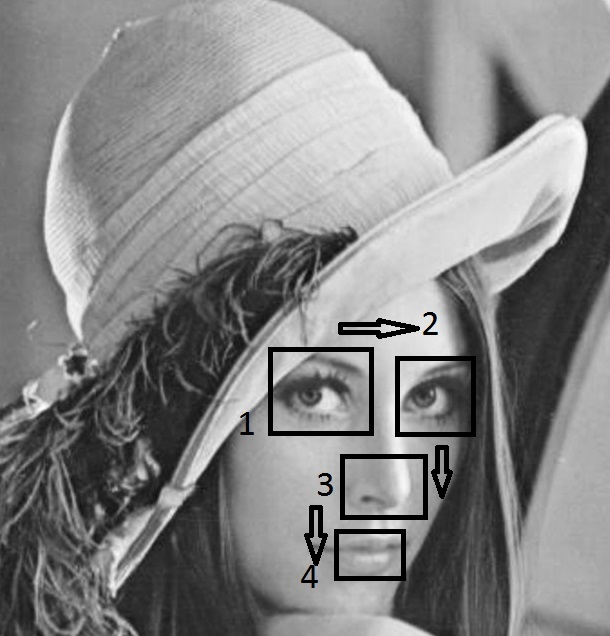
\includegraphics[width=0.5\textwidth]{misc/photos/face}
		\caption{Визуальная интерпретация каузальной матрицы. 1 обозначена область детектирования сенсора, отвечающего за левый глаз, 2 - за правый глаз, 3 - за нос и 4 - за рот. Стрелками обозначены временные переходы (саккады) от срабатывания одного сенсора к срабатыванию следующего.}		
	\end{figure}

	В вышеприведенном примере, каждый признак, составляющий образ знака <<лицо>>, также может представляться некоторым знаком в картине мира субъекта. Таким образом, случай, когда характерными признаками образа знака выступают данные с сенсоров, является частным. В более общей постановке, признаками, образующими образ знака, являются другие знаки, которые соответствуют этим характерным признакам. следовательно, мы можем сопоставить образу $p$ знака $s$ множество $S_p(s)$ мощности $q$, каждому элементу которого соответствует номер строки каузальной матрицы $z$ размера $q$ на $h$, т.е. каждому признаку $s_i\in S_p(s)$ соответствует характеристический бинарный вектор, задающий на местах единиц те дискретные моменты времени, в которые данный признак должен присутствовать во входных данных, чтобы успешно распознать образ знака (актуализировать знак) $s$. 
	
	Образу каждого знака может соответствовать несколько каузальных матриц, которые задают различные прецеденты наблюдения во внешней среде представляемого объекта или процесса. Весь кортеж каузальных матриц образа знака $s$ будем обозначать как $Z^p(s)$. 
		
	Для уточнения определения множества $S_p(s)$ введем семейство вложенных бинарных отношений $\{\sqsubset_p,\sqsubset_p^1,\sqsubset_p^2,\dots\}$, определённых на множестве знаков $S$. Будем считать, что знак $s_i$ \textit{является элементом образа} знака $s$, $(s_i,s)\in\sqsubset_p$ или $s_i\sqsubset_p s$, в том случае, если $s_i\in S_p(s)$. Если известно, что знаку $s_i$ соответствует единица в $t$-м столбце некоторой каузальной матрицы $z\in Z^p(s)$ знака $s$, то будем использовать отношение $\sqsubset_p^t$ такое, что  $\sqsubset_p^t\subset \sqsubset_p$.
	
	\subsection{Актуализация знака}
	
	Кратко опишем работу алгоритма распознавания образа знака (актуализации знака) по рис.~\ref{fig:percept}. Будем считать, что образы знаков сгруппированы по сходству множеств $S_p(s)$ в узлы, которые организованы в иерархические структуры (подробнее см. \cite{Panov2014d}). В узлы нижнего уровня входят каузальные матрицы знаков, которые являются признаками для знаков, чьи каузальные матрицы входят в узлы более высокого уровня. Такие узлы и каузальные матрицы образов знаков формируются в результате обучения \cite{Panov2014d,Skrynnik2016}, в данной версии алгоритма мы считаем, что все матрицы и узлы уже сформированы и не обновляются. Далее ограничимся тем случаем, когда все матрицы в рамках одного узла обладают одним и тем же количеством столбцов, что в ввиду схожести матриц в одном узле является естественным условием. Промежуток времени, в течение которого обрабатываются все колонки каузальных матриц узла называется вычислительным циклом данного узла.
	
	\begin{figure}
		\centering
		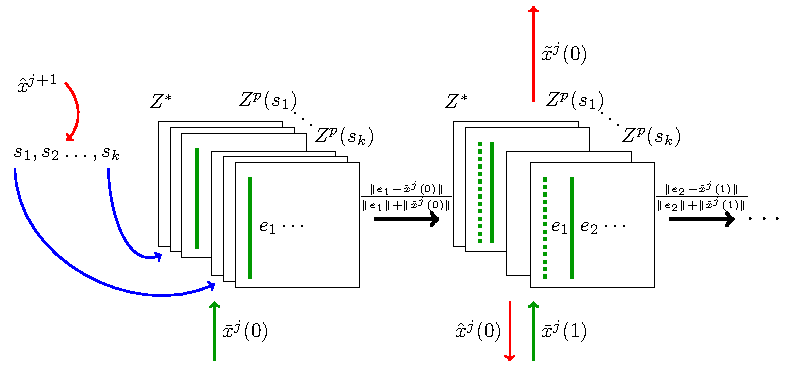
\includegraphics[width=0.8\textwidth]{algo/perception}
		\caption{Схема алгоритма распознавания образа знака}
		\label{fig:percept}		
	\end{figure}

	Вычислительный цикл распознавания в узле уровня $j$ начинается с определения начального состояния узла при помощи действительного вектора с верхнего уровня иерархии - вектора ожиданий $\hat x^{j+1}(\tau_s)$, формируемого на основе состояния узла верхнего уровня (шаги \ref{alst:init_start}--\ref{alst:init_end}) в момент времени $\tau_s$. Начальное состояние определяется как подмножество таких знаков, образы которых предсказываются на основе вектора ожиданий. Введем некоторую константу $c_1$, которая определяет порог предсказываемого веса распознаваемых образов, выше которого соответствующие каузальные матрицы попадают во множество активных матриц $Z^*$ (шаг \ref{alst:select_f}). Далее производится отбор тех каузальных матриц из множества активных, для которых обычное расстояние по норме $\|x\|=\sum_i |x_i|$ первого столбца $e_1$ от входного вектора $\bar x^j(0)$ в начальный момент времени не превышает некоторой константы $c_2$ (шаг \ref{alst:select_z}). Обновленное множество полученных таким образом активных каузальных матриц является текущим состоянием узла (шаг \ref{alst:init_state}). На основе активных каузальных матриц методом голосования вычисляется выходной вектор узла  в начальный момент времени $\tilde x^j(0)$ (шаги \ref{alst:init_calc_out2} -- \ref{alst:init_calc_out3}).

	\linespread{1}
	\begin{algorithm}[H]
		\label{alg:automato}
		\begin{algorithmic}[1]
					\Require $\tau_s, \hat x^{j+1}(\tau_s)$, $\omega^j$ - функция входов.
		\Ensure $\varphi^j$ - функция ожиданий, $\vec\eta^j$ - функция выходов.

		\State $F^*=\varnothing,Z^*=\varnothing,t=0$; 
		\State $c_1\in(0,1), c_2\in(0,1)$;

		\Statex \Comment{определение начального состояния}
				
		\ForAll{компонент $\hat x_k^{j+1}$ вектора $\hat x^{j+1}(\tau_s)=(\hat x_1^{j+1},\hat x_2^{j+1},\dots,\hat x_l^{j+1})$} \label{alst:init_start}
			\If{$\hat x_k^{j+1}{\ge}c_1$} \label{alst:select_f}
				\State $F^*=F^*\cup\{s_k\}$;
			\EndIf
		\EndFor
		
		\State $\bar x(0):=\omega^j(\tau_s)$;
		
		\ForAll{знаков $s_k\in F^*$}
			\ForAll{каузальных матриц $z\in Z^p(s_k)$}
				\If{$\frac{\|e_1-\bar x^j(0)\|}{\|e_1\|+\|x^j(0)\|}<c_2$} \label{alst:select_z}
					\State $Z^*:=Z^*\cup\{z\}$;
				\EndIf
			\EndFor
		\EndFor
		
		\State $Z^*$ - начальное состояние узла; \label{alst:init_state}
		\State $\bar N=(|\{z|z\in Z^*,z\in Z^p(s_1)\}|,\dots,|\{z|z\in Z^*,z\in Z^p(s_l)\}|)$; \label{alst:init_calc_out2}
		\State $\eta(0):=\tilde x^j=W(\bar N)$; \label{alst:init_calc_out3}
		\State $\varphi^j(0):=\hat x^j=W(\sum_{s_k\in F^*}\hat x_k^{j+1}\sum_{z\in Z^*}e_2(z))$;\label{alst:init_control}
		\label{alst:init_end}
			\algstore{algst:store1}
		\end{algorithmic}
	\end{algorithm}
	\linespread{2}

	Вектор ожиданий $\hat x^j(0)$ определяется как нормированный вектор, $s$-ый компонент которого равен сумме всех $s$-ых элементов вторых колонок активных каузальных матриц с весами, соответствующими элементам вектора ожиданий $\hat x^{j+1}(\tau_s)$ (шаг \ref{alst:init_control}). Т.к. используется представление о будущем входном сигнале (вторая колонка каузальных матриц), то $\hat x^j(0)$ является вектором ожиданий для нижнего уровня иерархии.

	\linespread{1}
	\begin{algorithm}[H]
		\begin{algorithmic}[1]
			\algrestore{algst:store1}
				\Statex \Comment{основной цикл}
	
	\State $t=1$;
	\While{$t\leqslant{h_i^j}-1$} \label{alst:cycle_start}
		\State $\bar{x}_i^j:=\omega(\tau_s+t)$;
	
		\ForAll{матриц предсказания $Z_r^k$ из множества $Z^*$}
			\If{$\frac{\|\bar{z}_{t+1}^r-\bar{x}_i^j\|}{\|\bar{z}_{t+1}^r\|+\|\bar{x}_i^j\|}\geqslant{c_2}$} \label{alst:update_z}
				\State $Z^*:=Z^*\setminus\{Z_r^k\}$;
			\EndIf
		\EndFor
	
		\State $\varphi_i^j(\bar x_i^j,\hat{x}_i^{j+1}(\tau_s)) := Z^*$; 
		\State $\bar N=(|\{Z_r^1|Z_r^1\in Z^*\}|,\dots,|\{Z_r^{l_i^j}|Z_r^{l_i^j}\in Z^*\}|)$; \label{alst:calc_out1}
		\State $\eta(Z^*)=\bar{x}_i^{*j}:=W(\bar N)$; \label{alst:calc_out3}
	
		\State $t=t+1$;
		\If{$t\leqslant{h}_i^j-2$}
			\State $\hat{x}_i^j:=W(\sum_{\hat f_k\in\hat F^*}\hat x_{ik}^{j+1}\sum_{Z_r^k\in Z^*}\bar z_t^r)$; \label{alst:calc_state1}
		\EndIf
	\EndWhile \label{alst:cycle_end}
	
	\Return $\varphi_{i\Delta t}^j,\vec\eta_{i\Delta t}^j$.
		\end{algorithmic}
	\end{algorithm}
	\linespread{2}
		
	После определения начального состояния начинает выполняться тело основного цикла, в котором до тех пор, пока время не превысит характерное время узла $h^j$ (число столбцов каузальных матриц) повторяется вычисление выходного вектора и состояния в следующий момент времени (шаги \ref{alst:cycle_start}--\ref{alst:cycle_end}). В начале этого этапа обновляется состояние, т.е. множество активных каузальных матриц $Z^*$, за счёт удаления тех матриц, соответствующие столбцы которых достаточно сильно отличаются от текущего входного вектора $\bar x^j(t)$ (шаг \ref{alst:update_z}). Далее методом голосования по количеству матриц в множестве активных каузальных матриц, отвечающих за соответствующий образ, вычисляется выходной вектор $\tilde x^j(t)$ (шаги \ref{alst:calc_out1}--\ref{alst:calc_out3}).

	В завершение тела основного цикла вычисляется выходной вектор ожиданий в следующий момент времени $\hat x^j(t)$. Вектор ожиданий равен нормированному вектору, элементы которого равны сумме элементов столбцов всех активных кауазальных матриц, соответствующих текущему моменту времени с учётом весов начального вектора ожиданий $\hat x^{j+1}(\tau_s)$ (шаг \ref{alst:calc_state1}).

	\subsection{Каузальная сеть}
	
	Введем специальную процедуру $\Lambda_p: 2^Z\rightarrow 2^{\mathbb N}\times 2^{\mathbb N}$, которая каждому кортежу каузальных матриц $Z^p(s)\subset Z$ образа знака $s$ ставит в соответствие два не пересекающихся подмножества индексов столбцов $I^c\subset\mathbb N, \forall i\in I^c\ i\leq h$ и $I^e\subset\mathbb N, \forall i\in I^e\ i\leq h$ : $\Lambda_p(Z^p(s))=(I^c,I^e)$ таких, что $I^c\cap I^e=\varnothing$. Множество $I^c$ будем называть индексами столбцов условий, а множество $I^e$ - индексами столбцов эффектов. Например, если для кортежа матриц $Z=\{((1, 0), (0, 1))\}$ процедура $\Lambda_p$ выдает два множества $\{1\}$ и $\{2\}$, то это означает, что появление признака, соответствующего первой строке матрицы, вызывает появление признака, соответствующего второй строке. Процедура $\Lambda_p$, таким образом, устанавливает причинно-следственное отношение на множестве входных событий и может реализовываться различными способами, в т.ч. на основе алгоритмов Норриса, FCO и др. (см. \cite{Kuznetsov2001})
	

	В том случае, когда для матриц $Z^p(s)$ образа знака $s$ множество столбцов эффектов не пусто $I^e \not=\varnothing$, будем считать, что знак представляет некоторое действие или процесс, результат которого кодируется в столбцах эффектов, а условие - в столбцах условий (соответствующий знак является процедурным). В противном случае, когда для матриц $Z^p(s)$ образа знака $s$ множество столбцов эффектов пусто $I^e=\varnothing$, т.е. когда по данному кортежу каузальных матриц невозможно однозначно определить, какие события предшествуют другим, будем считать, что причинно-следственная связь не установлена и знак представляет некоторый объект или ситуацию (соответствующий знак является объектным). 

	\begin{figure}[H]
		\centering
		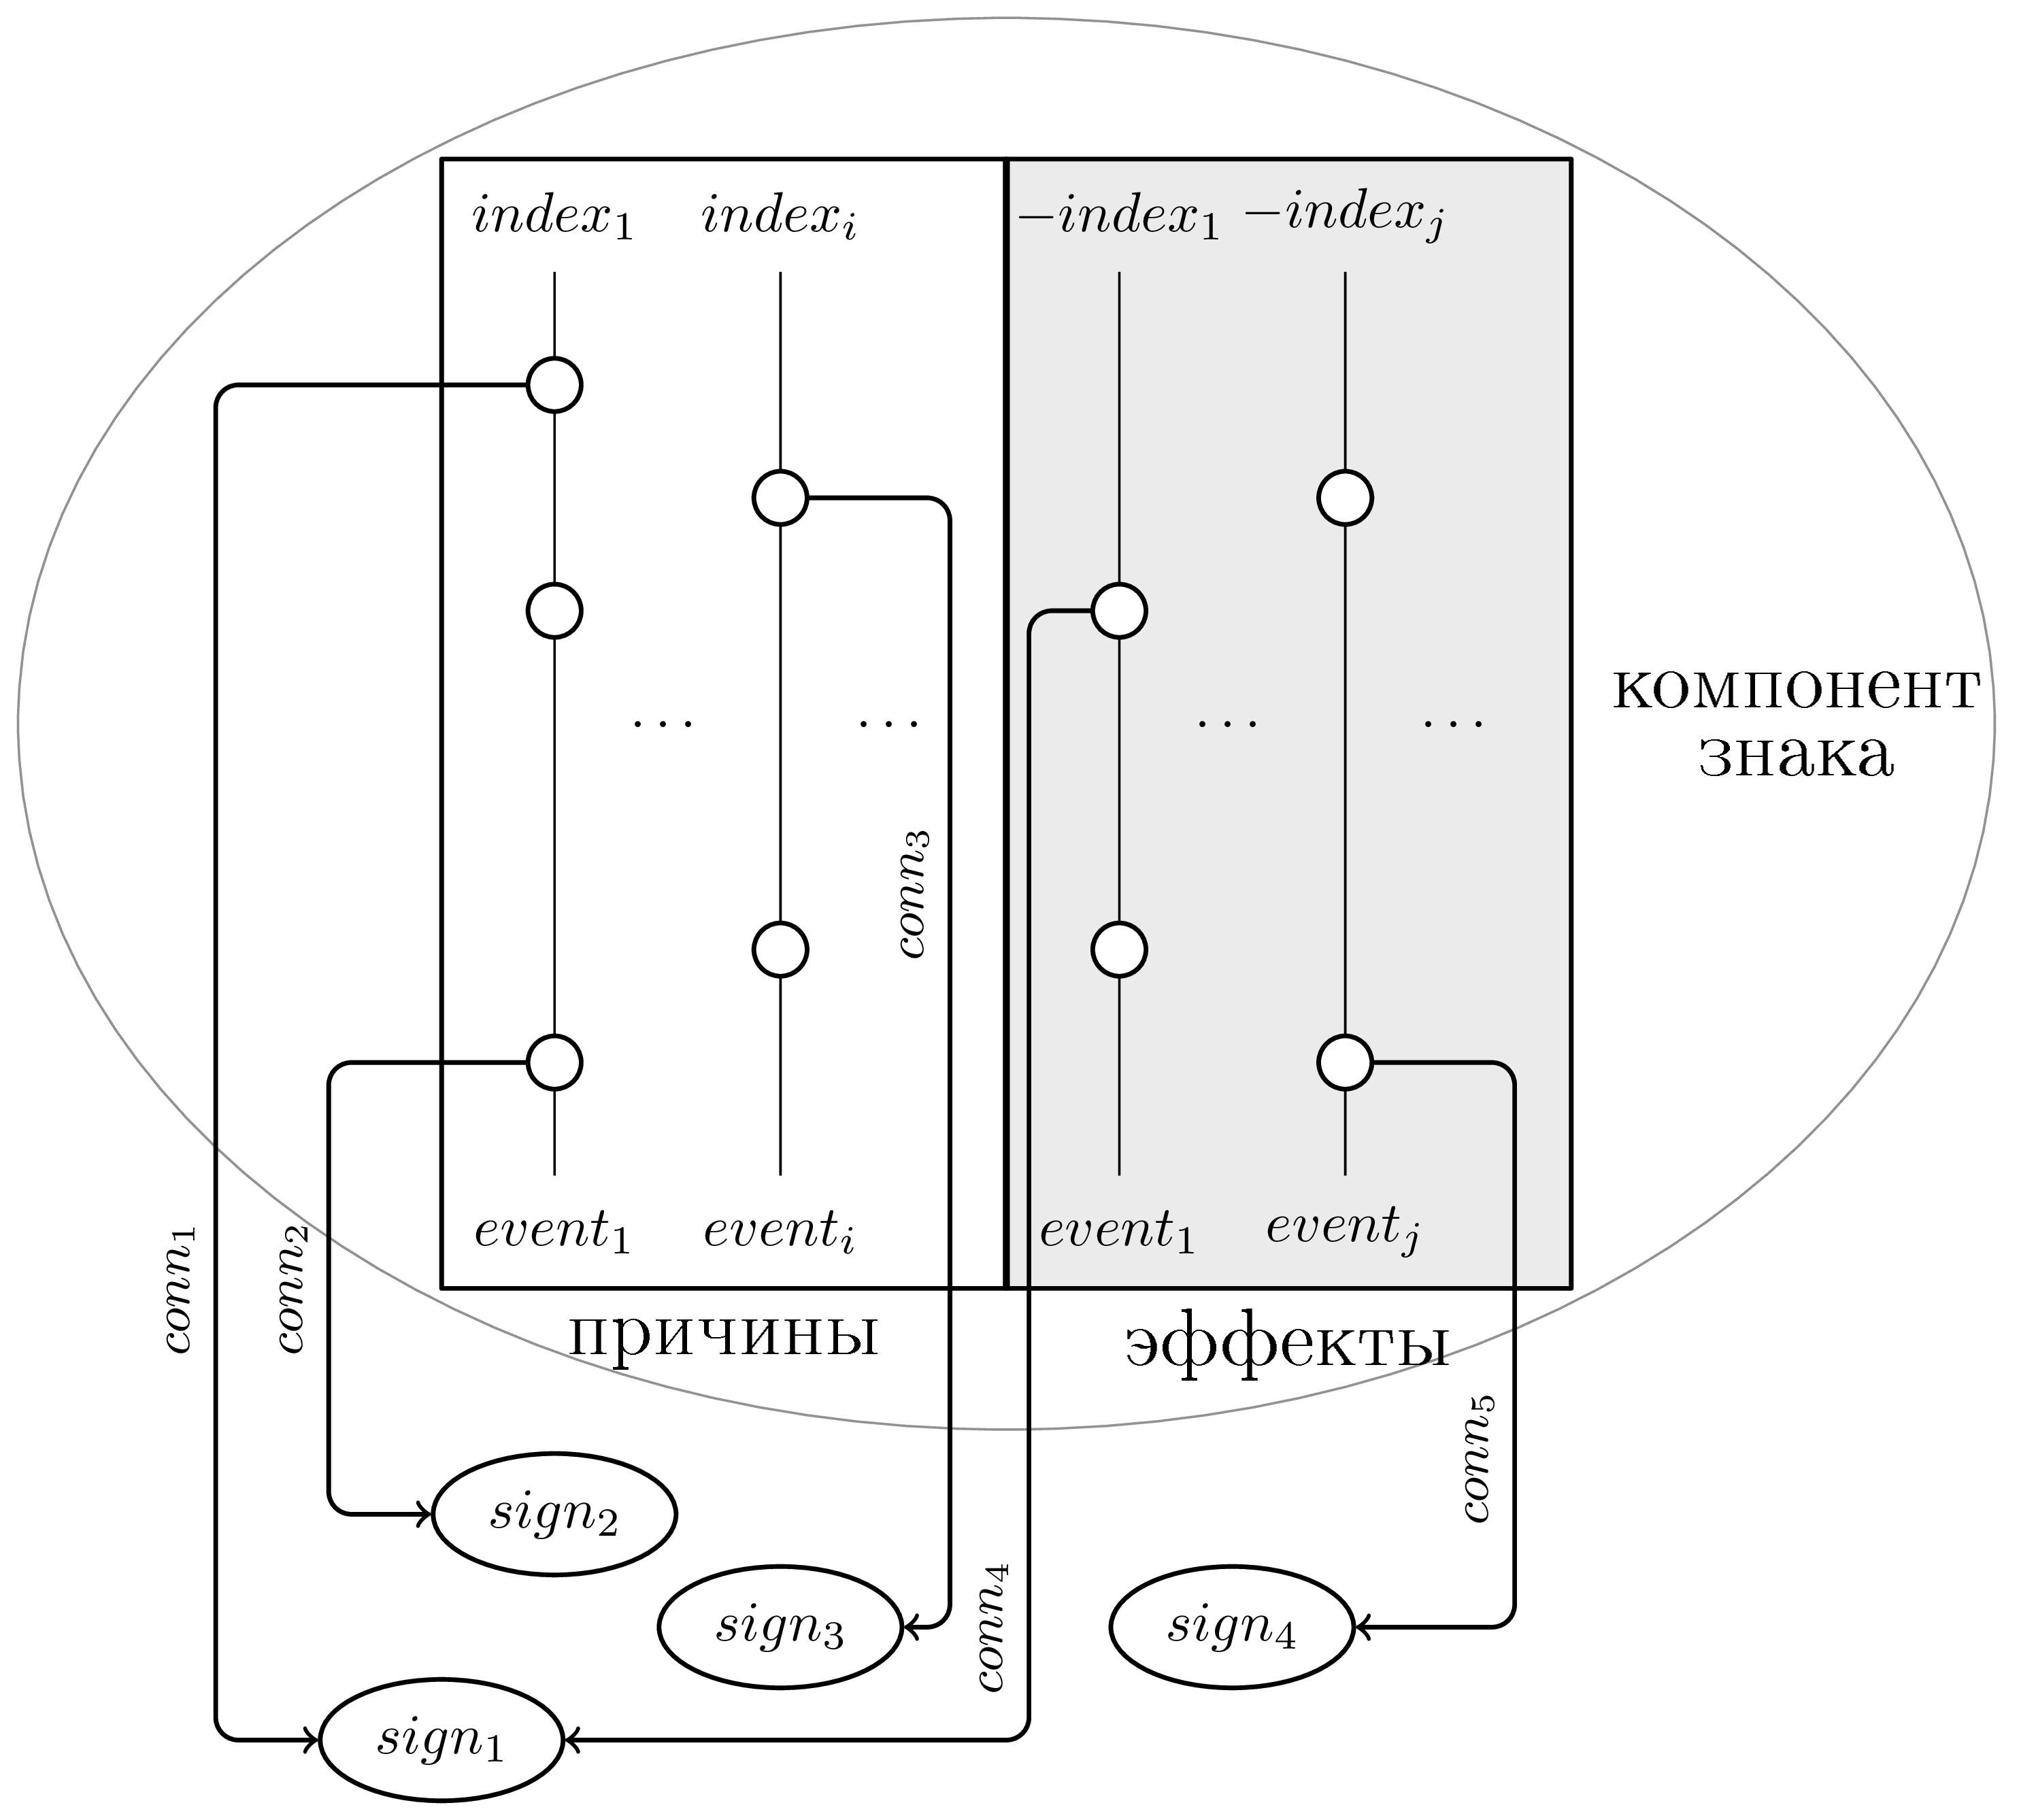
\includegraphics[width=0.6\textwidth]{causnet/caus_matr_ru}
		\caption{Пример каузальной матрицы}	
		\label{fig:caus_matr}	
	\end{figure}
	
	Справедливы следующие утверждения относительно свойств процедуры $\Lambda_p$:
	\begin{itemize}
		\item $I^c\cap I^e=\varnothing$ --- столбец каузальной матрицы не может быть одновременно и условием и эффектом,
		\item $|I^c\cup I^e|=h$ --- других типов столбцов, кроме столбцов условий и эффектов, нет,
		\item $I^c\not = \varnothing$ --- среди столбцов каузальной матрицы должен быть хотя бы один столбец условий, в то время как эффектов может и не быть (в случае объектных признаков),
		\item $\forall i\in I^e, j\in I^c\ i>j$ --- все условия предшествуют эффектам по времени.
	\end{itemize}
	
	Переходя к нотации, принятой в искусственном интеллекте, можем считать, что каузальная матрица $z$ образа знака $s$ является правилом $r=(F_C(z),F_A(z),F_D(z))$ \cite{Osipov2008b}, в котором:
	\begin{itemize}
		\item $F_C (z)\subseteq S_p(s)$ --- множество признаков - условий правила: $\forall f\in F_C(z)$ $f\sqsubset_p^i s, i\in I^c$;
		
		\item $F_A(z)\subseteq S_p(s)$ --- множество добавляемых правилом признаков: $\forall f\in F_A(z)$ $f\sqsubset_p^i s,i\in I^e, f\not\sqsubset^j f_p, j\in I^c$;
		
		\item $F_D(z)\subseteq S_p(s)$ --- множество удаляемых правилом признаков: $\forall f\in F_D(z)$ $f\not\sqsubset^i s, i\in I^e,f\sqsubset^j s, j\in I^c$.
	\end{itemize}

	Пример каузальной матрицы, с учетом выше сказанного, приведен на рис. \ref{fig:caus_matr}.
	
	Теперь введем понятие каузальной сети, которая будет определять гетерархию на множестве образов. Каузальная сеть $W_p=\langle V_p, E_p \rangle$ - является помеченным ориентированным графом, в котором
	\begin{itemize}
		\item каждому узлу $v\in V_p$ ставится в соответствие кортеж каузальных матриц $Z^p(s)$ образа некоторого знака $s$, что будем обозначать как $v\rightarrow Z^p(s)$;
		\item ребро $e=(v_1, v_2)$ принадлежит множеству ребер графа $E$, если $v_1\rightarrow Z^p(s_1), v_2\rightarrow Z^p(s_2)$ и $s_1\in S_p(s_2)$, т.е. если знак $s_1$ является элементом образа $s_2$;
		\item каждому ребру графа $e=(v_1, v_2), v_1\rightarrow Z^p(s_1), v_2\rightarrow Z^p(s_2)$ ставится в соответствие метка $\epsilon=(\epsilon_1,\epsilon_2,\epsilon_3)$ - кортеж трех натуральных чисел:
		\begin{itemize}
			\item $\epsilon_1$ - индекс исходной матрицы в кортеже $Z^p(s_1)$, может принимать специальное значение 0, если исходными могут служить любые матрицы из кортежа;
			\item $\epsilon_2$ - индекс целевой матрицы в кортеже $Z^p(s_2)$, строка которой ставится в соответствие признаку $s_1$;
			\item $\epsilon_2$ - индекс столбца в целевой матрице, в которой в соответствующей признаку $s_1$ строке стоит 1, может принимать положительные значения (столбцы условий) и отрицательные (столбцы эффектов).
		\end{itemize}		
	\end{itemize}
	
	Пример такой сети изображен на рис. \ref{fig:caus_net}.

	\begin{figure}[h]
		\centering
		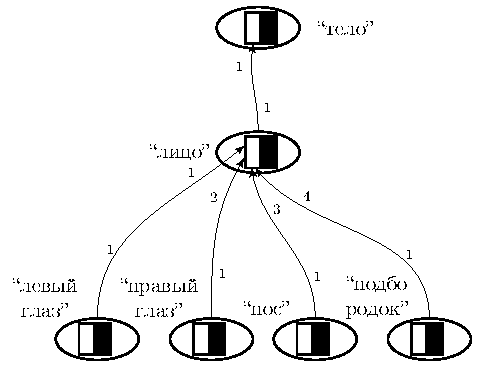
\includegraphics[width=0.5\textwidth,page=1]{examples/causnet/caus_net}
		\caption{Схема каузальной сети. Здесь каузальные матрицы изображены в виде квадратов, столбцы условий - левая белая часть квадрата, столбцы эффектов - черная правая часть квадратов. Метка $\epsilon_1$ отображается в начале каждой стрелки, метка $\epsilon_2$ определяется как номер квадрата, к которому идет стрелка, а метка $\epsilon_3$ отображается в конце каждой стрелки.}
		\label{fig:caus_net}		
	\end{figure}
		
	Аналогичным образом определяются каузальные сети для остальных компонент знака - для значения и личностного смысла. Для каждого знака $s$ задаются множества $S_m(s)$ и $S_a(s)$, т.е. определяются семейства вложенных отношений $\{\sqsubset_m,\sqsubset_m^1,\sqsubset_m^2,\dots\}$ - \textit{являться элементом значения}, и $\{\sqsubset_a,\sqsubset_a^1,\sqsubset_a^2,\dots\}$ - \textit{являться элементом смысла}. Множество $S_m(s)$ интерпретируется как ролевой состав знака $s$, например, элементы подкласса или роль действия. Множество $S_a(s)$ интерпретируется как мгновенный компонентный состав некоторой ситуации, наблюдаемой и переживаемой субъектом, носителем картины мира, в настоящее время. Аналогично определяются множества $Z^m(s)$, $Z^a(s)$, процедуры $\Lambda_m$ и $\Lambda_a$.
	
	Три типа каузальных сетей отличаются друг от друга отношениями, которые генерируются на основе этих сетей для соответствующего множества компонент знаков, операциями, которые выполняются на этих сетях, и той ролью, которую они играют при реализации когнитивных функций, например, планирования поведения \cite{Osipov2015d}. Теперь мы можем дать формальное определение знака \cite{Osipov2015c} с использованием введенного формализма каузальных матриц и каузальных сетей.
	
	\begin{definition}
		Знаком будем называть четверку $s=\langle n, p, m, a \rangle$, где $n$ - имя знака, $p=Z^p$ - образ знака, т.е. кортеж каузальных матриц, которым соответствует некоторый узел каузальной сети на образах с учетом всех входящих и исходящих связей, $m=Z^m$ - значение знака, т.е. кортеж каузальных матриц, которым соответствует некоторый узел каузальной сети на значениях  с учетом всех входящих и исходящих связей, $a=Z^a$ - образ знака, т.е. кортеж каузальных матриц, которым соответствует некоторый узел каузальной сети на личностных смыслах  с учетом всех входящих и исходящих связей.
	\end{definition}
	
	Далее мы будем считать, что каждый знак обладает значением, т.е. $Z^m\not = \varnothing, S_m\not=\varnothing$. В том случае, когда у знака нет образа, т.е. $Z^p=\varnothing,S_p=\varnothing$, будем называть такой знак \textit{абстрактным}. Наконец, в том случае, когда у знаку не присвоен личностный смысл, т.е. $Z^a=\varnothing, S_a=\varnothing$, будем называть его \textit{безличным}.
	
	\section{Семиотическая сеть}
	
	Далее определим три семейства бинарных отношений на множестве знаков, которые  генерируются на основе структуры фрагментов трех типов каузальных сетей, к которым принадлежат соответствующие компоненты знаков.
		
	\subsection{Отношения на множестве образов}	
	
	Начнем с определения отношений на множестве знаков, генерируемых на основе каузальной сети на образах. Для этого потребуется определения равенства, сходства, включения и противопоставления двух каузальных матриц:
	
	\begin{definition}
		Две каузальных матрицы $z_1$ и $z_2$ равны ($z_1=z_2$) тогда и только тогда, когда размерности матриц равны, множества индексов столбцов эффектов и условий совпадают $\Lambda({z_1})=\Lambda({z_2})$ и каждый бинарный вектор $e_t^1$, столбец матрицы $z_1$, равен соответствующему по порядку бинарному вектору $e_t^2$, столбцу матрицы $z_2$.
	\end{definition}
	
	\begin{definition}
		Две каузальных матрицы $z_1$ и $z_2$ обладают сходством ($z_1\sim z_2$) тогда и только тогда, когда  существуют такие два бинарных вектора $e_i$ и $e_j$, столбца матриц $z_1$ и $z_2$, что их покомпонентное произведение (т.е. произведение тех компонент, которые соответствуют одному и тому же признаку, если соответствующего признака в векторе нет - считается, что на его месте стоит ноль) не равно нулевому вектору $e_i*e_j\not =\varnothing$ и они одновременно являются либо столбцами условий $i\in I^c(z_1), j\in I^c(z_2)$, либо столбцами эффектов $i\in I^e(z_1), j\in I^e(z_2)$.
	\end{definition}
	
	\begin{definition}
		Каузальная матрица $z_1$ включена в каузальную матрицу $z_2$ ($z_1\subseteq z_2$) тогда и только тогда, когда  для любого бинарного вектора $e_i$, столбца матрицы $z_1$, существует бинарный вектор $e_j$, столбец матрицы $z_2$, такой, что $e_i | e_j=e_j$ ($|$ - операция побитового <<или>>) и они одновременно являются либо столбцами условий $i\in I^c(z_1), j\in I^c(z_2)$, либо столбцами эффектов $i\in I^e(z_1), j\in I^e(z_2)$.
	\end{definition}
	
	\begin{definition}
		Две каузальных матрицы $z_1$ и $z_2$ противопоставлены друг другу ($z_1\perp z_2$) тогда и только тогда, когда размерности матриц равны, множества индексов столбцов эффектов и условий совпадают $\Lambda({z_1})=\Lambda({z_2})$ и каждый бинарный вектор $e_t^1$, столбец матрицы $z_1$, не имеет пересечения с соответствующим ему по порядку бинарным вектором $e_t^2$, столбцом матрицы $z_2$, т.е. $e_t^1\& e_t^2=e_0$, где $\&$ - операция побитового <<и>>, а $e_0$ - нулевой вектор той же длины, что и вектора $e_t^1$ и $e_t^2$.
	\end{definition}
	
	Кроме уже введенного ранее семейства вложенных отношений <<являться элементом образа>> ${\sqsubset_p,\sqsubset_p^1,\dots}$, на основе определений отношений на множестве каузальных матриц, зададим четыре отношения на множестве знаков $S$.
	\begin{definition}
		Пара знаков  $s_1$ и $s_2$ принадлежит \textbf{отношению эквивалентности по образам} $R_1^p$, $(s_1,s_2)\in R_1^p$, если мощность кортежа $Z^p(s_1)=(z_1^1,z_2^1,...)$ равна мощности кортежа $Z^p(s_2)=(z_1^2,z_2^2,...)$ и каждая каузальная матрица первого кортежа равна соответствующей по порядку матрице второго кортежа, т.е. $|Z^p(s_1)| = |Z^p(s_2)|, \forall z_t^1\in Z^p(s_1)\ \exists z_t^2\in Z^p(s_2): z_t^1=z_t^2$.
	\end{definition}
	
	\begin{definition}\label{def:sim}
		Пара знаков  $s_1$ и $s_2$ принадлежит \textbf{отношению сходства по образу} $R_2^p$, $(s_1,s_2)\in R_2^p$, если для каждой каузальной матрицы $z_i$ кортежа $Z^p(s_1)$ в кортеже $Z^p(s_2)$ найдется такая матрица $z_j$, что $z_i$ обладает сходством с $z_j$, т.е. $\forall z_i\in Z^p(s_1)\ \exists z_j\in Z^p(s_2): z_i\sim z_2$.
	\end{definition}
	
	\begin{definition}
		Пара знаков  $s_1$ и $s_2$ принадлежит \textbf{отношению включения по образу} $R_3^p$, $(s_1,s_2)\in R_3^p$, если для каждой каузальной матрицы $z_i$ кортежа $Z^p(s_1)$ в кортеже $Z^p(s_2)$ найдется такая матрица $z_j$, что $z_i$ будет включена в $z_j$, т.е. $\forall z_i\in Z^p(s_1)\ \exists z_j\in Z^p(s_2): z_i\subseteq z_2$.
	\end{definition}

	\begin{definition}
		Пара знаков  $s_1$ и $s_2$ принадлежит \textbf{отношению противопоставления по образу} $R_4^p$, $(s_1,s_2)\in R_4^p$, если мощность кортежа $Z^p(s_1)=(z_1^1,z_2^1,...)$ равна мощности кортежа $Z^p(s_2)=(z_1^2,z_2^2,...)$ и каждая каузальная матрица первого кортежа противопоставлена соответствующей по порядку матрице второго кортежа, т.е. $|Z^p(s_1)| = |Z^p(s_2)|, \forall z_t^1\in Z^p(s_1)\ \exists z_t^2\in Z^p(s_2): z_t^1\perp z_t^2$.
	\end{definition}
	
	Таким образом, семейство отношений $R^p$ на множестве образов состоит из отношений <<являться элементом образа>>, эквивалентности, сходства, включения и противопоставления по образу.
		
	\subsection{Отношения на множестве значений}	
	
	К семейству отношений $R^m$ на множестве значений отнесем вложенные отношения <<являться элементом значения>> ${\sqsubset_m,\sqsubset_m^1,\dots}$ и аналогичные случаю с образами - отношения эквивалентности $R_1^m$, сходства $R_2^m$, включения $R_3^m$ и противопоставления $R_4^m$ по значению.
	
	Кроме того, важную роль на сети значений при моделировании когнитивных функций играют следующие два отношения: отношение классификации $R_5^m$, причинно-следственное отношение $R_6^m$ и сценарное отношение $R_7^m$.
	
	\begin{definition}
		Пара знаков $s_1$ и $s_2$ принадлежит \textbf{отношению классификации} $R_5^m$, $(s_1,s_2)\in R_5^m$, если $s_1$ - абстрактный объектный знак и существует только одна каузальная матрица значения знака $s_1$ с единственным столбцом, в котором только одна единица, соответствующая знаку $s_2$, т.е. $Z^p(s_1)=\varnothing, I^e(s_1)=\varnothing, \exists z\in Z^m(s_1): h(z)=1, |e_1(z)|=1, s_2\sqsubset_m^1 s_1$.
	\end{definition}
	
	\begin{definition}
		Пара знаков $s_1$ и $s_2$ принадлежит \textbf{сценарному отношению} $R_6^m$, $(s_1,s_2)\in R_6^m$, если $s_1$ - процедурный знак, $s_2$ - объектный знак, возможно, абстрактный, и знак $s_2$ является элементом значения знака $s_1$, т.е. $I^e(s_1)\not = \varnothing, I^e(s_2) = \varnothing, s_2\sqsubset_m s_1$.
	\end{definition}
	
	Примеры элементов отношений $R_5^m$ и $R_6^m$ приведены на рис.\ref{fig:signif_relat}.
	
	\begin{figure}[h]
		\centering
		\includegraphics[width=0.7\textwidth,page=2]{examples/causnet/caus_net}
		\caption{Пример элементов отношений на каузальной сети значений. Здесь $R_5^m=\{(s_2,s_3),(s_2,s_4),(s_2,s_5),(s_2,s_6),(s_1,s_2)\}$, $R_6^m=\{(s_7,s_1),(s_7,s_8),(s_7,s_9)\}$. Условные обозначения те же, что и на рис.\ref{fig:caus_net}.}
		\label{fig:signif_relat}		
	\end{figure}
	
	\subsection{Отношения на множестве личностных смыслов}	
	К семейству отношений $R^a$ на множестве личностных смыслов отнесем вложенные отношения <<являться элементом смысла>> ${\sqsubset_a,\sqsubset_a^1,\dots}$ и аналогичные случаю с образами - отношения эквивалентности $R_1^a$, сходства $R_2^a$, включения $R_3^a$ и противопоставления $R_4^a$ по смыслу.
	
	Также на множестве личностных смыслов введем ситуационное отношение $R_5^a$.

	\begin{definition}
		Пара знаков $s_1$ и $s_2$ принадлежит \textbf{ситуационному отношению} $R_5^a$, $(s_1,s_2)\in R_5^a$, если $s_1$ - процедурный знак, $s_2$ - не абстрактный объектный знак, и знак $s_2$ является элементом смысла знака $s_1$, т.е. $I^e(s_1)\not = \varnothing, I^e(s_2) = \varnothing, S_p(s_2)=\varnothing, s_2\sqsubset_a s_1$.
	\end{definition}
	
	На основе определения ситуационного отношения можно ввести понятия ситуации как некоторый процедурный знак со всеми не абстрактными объектными знаками, в паре с которыми он принадлежит ситуационному отношению.
	
	\begin{definition}
		Множество знаков $Sit=\{s_1,s_2,\dots,s_n\}$ будем называть \textit{ситуацией}, если $s_1$ - единственный процедурный знак в множестве $Sit$ и для всех $1<i\leq n\ s_i\in Sit, (s_1,s_i)\in R_5^a$.
	\end{definition}
	
	Пример элементов отношения $R_5^a$ и ситуации приведен на рис.\ref{fig:mean_relat}

	\begin{figure}[h]
		\centering
		\includegraphics[width=0.7\textwidth,page=3]{examples/causnet/caus_net}
		\caption{Пример элементов отношения $R_5^a$ на каузальной сети смыслов. Здесь $R_5^a=\{(s_5,s_1),(s_5,s_2),(s_5,s_3),(s_5,s_4)\}$, что эквивалентно следующей ситуации <<Иван рисует трапецию карандашом>>. Условные обозначения те же, что и на рис.\ref{fig:caus_net}.}
		\label{fig:mean_relat}		
	\end{figure}
			
	\subsection{Семиотическая сеть}
	Будем называть \textit{семиотической сетью} пятерку $\Omega=\langle W_p, W_m, W_a, R, \Theta \rangle$, где
	\begin{itemize}
		\item $W_p, W_m, W_a$ - соответственно каузальные сети на множестве образов, значений и личностных смыслах,
		\item $R$ - семейство отношений на множестве знаков, сгенерированных на основе трех каузальных сетей, т.е. $R=\{R^p, R^m, R^a\}$,
		\item $\Theta$ - семейство операций на множестве знаков, которые будут определены ниже.
	\end{itemize} 
	

	\section{Операции в семиотической сети}
	Мы определим ряд операций, которые функционируют в картине мира и генерируют новый знак на основе компонент двух входных знаков. Другими словами, генерация, например, нового образа на основе двух образов других знаков, влечет за собой формирование остальных компонент нового знака по определенным правилам, которые определяются данной операцией. Возможно описать целый ряд подобного рода операций, но в данной работе будут даны определения только для основных их них для каждой каузальной сети. Для простоты изложения будем далее считать, что каждая компонента знака характеризуется только одной каузальной матрицей. Также далее будет использована процедура образования нового знака, описанная в \cite{Osipov2014c}, которую здесь будем обозначать через $\Psi$.
	
	\subsection{Операция обобщения}
	
	Обобщение является одним из ключевых когнитивных процессов, которые позволяют организовывать знания в иерархической форме, формировать компактные представления объектов и процессов действительности. Психологи выделяют три вида обобщения: синкрет, комплекс и понятие \cite{Vygotsky1999}. При синкретическом обобщении ведущую роль играет личностный смысл знаков, т.е. субъективное отношение носителя картины мира к представляемым объектам. При формировании обобщения-комплекса используются образы знаков, объективно существующие признаки. Обобщение-понятие, основываясь на значении знаков, формируется уже в процессе рассмотрения родо-видовых отношений, знания о которых согласованы с другими участниками совместной деятельности.
	
	Определим операцию \textit{обобщения по образу} $\Theta^p: S\times S\rightarrow S$. Пусть $s_1=\langle n_1, \{z_1^p\}, \{z_1^m\}, \{z_1^a\} \rangle$, $s_2=\langle n_2, \{z_2^p\}, \{z_2^m\}, \{z_2^a\} \rangle$ - знаки такие, что $(s_1,s_2)\in R_1^p$, т.е. принадлежат отношению сходства. Новый образуемый знак обозначим через $s_3$. 
	
	По определению $\autoref{def:sim}$ это означает, что $z_1^p\sim z_2^p$, т.е. каузальные матрицы обладают сходством. Определим новую каузальную матрицу $z_3^p$ следующим образом: $z_3^p=(e_1^3,e_2^3,\dots,e_h^3)$, где для каждого столбца $e_i^3$ найдется пара столбцов $e_j^1, e_k^2$ матриц $z_1^p$ и $z_2^p$ соответственно, таких, что $e_i^3=e_j^1*e_k^2\not=\varnothing$ и $i\in I^c(z_3^p), j\in I^c(z_1^p), k\in I^c(z_2^p)$. Иными словами матрица $z_3^p$ является обобщением матриц $z_1^p$ и $z_2^p$ и содержит только те события, которые являются обобщением событий для обоих матриц.
	
	Пусть $Z'_1$ и $Z'_2$ - множества процедурных каузальных матриц, для которых знаки $s_1$ и $s_2$ соответственно являются признаками. Найдем среди этих двух множеств пару каузальных матриц, обладающих сходством: $(z_1^m,z_2^m)$. Далее определим процедурную каузальную матрицу $z_4^m$ - новую матрицу в каузальной сети значений, которая будет являться обобщением матриц $z_1^m$ и $z_2^m$: $z_4^m=(e_1^4,e_2^4,\dots)$, где для каждого столбца $e_i^4$ найдется пара столбцов $e_j^1, e_k^2$ матриц $z_1^m$ и $z_2^m$ соответственно, таких, что
	\begin{itemize}
		\item в каждом из них ссылка на соответствующие значения знаков $s_1$ и $s_2$ заменена на ссылку на значение c единственной пустой матрице $z_3^m$ вновь образуемого знака $s_3$,
		\item $e_i^4=e_j^1*e_k^2\not=\varnothing$ и 
		\item либо одновременно $i\in I^c(z_4^m), j\in I^c(z_1^m), k\in I^c(z_2^m)$, 
		\item либо одновременно $i\in I^e(z_4^m), j\in I^e(z_1^m), k\in I^c(z_2^m)$.
	\end{itemize}
	
	По сгенерированной паре матриц $z_3^p$ и $z_3^m$ с помощью процедуры образования нового знака $\Psi$ в результате операции $\Theta^p$ получаем новый знак $s_3$, образ которого является обобщением образов знаков $s_1$ и $s_2$, а значением является некоторая роль в обобщенном действии, выполняемом как со знаком $s_1$, так и со знаком $s_2$. Вновь образованная процедурная матрица $z_4^m$ может быть включена в один из существующих узлов на сети значений, либо послужить отдельным узлом нового знака, представляющего новое обобщенное действие.
	
	Приведем пример работы операции обобщения по образу. Пусть есть два знака $s_1$ и $s_2$ с именами \textit{<<яблоко>>} и \textit{<<апельсин>>} соответственно. Каузальные матрицы для образных компонент знаков $s_1$ и $s_2$ выглядят следующим образом (вместо единиц в матрице указаны имена признаков):
	\[
	z_1^p = \begin{bmatrix}
	0&0& \text{<<зеленый>>} \\
	0& \text{<<круглый>>} &0 \\
	\text{<<кожура>>} &0 &0  \\
	\text{<<тонкий>>} &0 &0
	\end{bmatrix}
	z_2^p = \begin{bmatrix}
	0&0& \text{<<оранжевый>>} \\
	0& \text{<<круглый>>} &0 \\
	\text{<<кожура>>} &0 &0  \\
	\text{<<толстый>>} &0 &0
	\end{bmatrix}
	\]
	Компоненты значений знаков $s_1$ и $s_2$ связаны по каузальной сети с процедурными знаками $s_3$ <<чистить яблоко>> и $s_4$ <<чистить апельсин>> (здесь вертикальной чертой отделены столбцы условий и эффектов):
	\[
	z_3^m= \left[\begin{array}{ccc|cccc}
	0&0&0&0&\text{<<стол>>}&0\\
	0&\text{<<яблоко>>}&0& 0&0&\text{<<яблоко>>}\\
	0&0& \text{<<нож>>} &0 &0\\
	0& 0& 0 &\text{<<на>>} &0&0\\
	\text{<<вплотную>>}& 0& 0 &0 &0&0\\
	\text{<<кожура>>} &0 &0 &\text{<<кожура>>}  &0&0\\
	\text{<<тонкий>>} &0 &0 & \text{<<тонкий>>} &0&0
	\end{array}
	\right]
	\]
	\[
	z_4^m= \left[\begin{array}{ccc|cccc}
	0&0&0&0&\text{<<стол>>}&0\\
	0&\text{<<апельсин>>}&0& 0&0&\text{<<апельсин>>}\\
	0&0& \text{<<пальцы>>} &0 &0&0\\
	0& 0& 0 &\text{<<на>>} &0&0\\
	\text{<<вплотную>>}& 0& 0 &0 &0&0\\
	\text{<<кожура>>} &0 &0 &\text{<<кожура>>}  &0&0\\
	\text{<<толстый>>} &0 &0 & \text{<<толстый>>} &0&0
	\end{array}
	\right]
	\] 
	В результате выполнения операции обобщения по образу $\Theta^p$ формируются два знака: обобщенный по признакам образа знак $s_5$ с именем <<фрукт>> и обобщенный по признакам значения знак $s_6$ чистить, представляющий собой обобщенное действие, которое можно выполнить с фруктом:
	
	\[
	z_5^p = \begin{bmatrix}
	0& \text{<<круглый>>} \\
	\text{<<кожура>>} &0
	\end{bmatrix}
	\]
	\[
	z_6^m= \left[\begin{array}{ccc|cccc}
	0&0&0&0&\text{<<стол>>}&0\\
	0&\text{<<фрукт>>}&0& 0&0&\text{<<фрукт>>}\\
	0& 0& 0 &\text{<<на>>} &0&0\\
	\text{<<вплотную>>}& 0& 0 &0 &0&0\\
	\text{<<кожура>>} &0 &0 &\text{<<кожура>>}  &0&0\\
	\end{array}
	\right]
	\] 
	
	\subsection{Операция замыкания по значению}
	Другой важной когнитивной функцией является способность формировать возможные сценарии на основе значений знаков. Особую роль этот процесс играет в житейской картине мира, где большинство когнитивных процессов, формирующих поведение человека, таких как планирование, коммуникация, основываются на нахождении, применении и образовании новых сценариев \cite{Chudova2012b,Osipov2015d}. Под сценарием в простейшем случае подразумевается некоторое действие, в котором зафиксированы исполнители той или иной роли, т.е. сценарий является специфицированным действием. Формально сценарием будем называть множество знаков $Scen=\{s_1,s_2,\dots, s_n\}$, в котором единственным процедурным знаком является $s_1$, а все остальные знаки образуют две подгруппы $S_r$ - множество знаков-ролей и $S_o$ - множество знаков-участников сценария. Знаки-роли из множества $S_r$ - это абстрактные знаки, которые связаны с $s_1$ сценарным отношением $R_6^m$. Знаки-участники из множества $S_o$ - это либо не абстрактные знаки, связанные с $s_1$ сценарным отношением $R_6^m$, либо знаки, которые в паре с другим знаком из множества $S_r$ принадлежат отношению классификации $R_5^m$.
	
	Определим операцию \textit{замыкания по значению} $\Theta^m$, которая по некоторому процедурному знаку $s$ формирует сценарий $Scen$: $\Theta^m(s)=Scen$. По сути формирование сценария заключается в итерационном включении знаков в множество $Scen$ при рассмотрении элементов отношений $R_5^m$ и $R_6^m$:
	
	\begin{itemize}
		\item[Шаг 1.] Включить в сценарий $Scen$ процедурный знак $s$: $Scen=\{s\}$.
		\item[Шаг 2.] Пополнить сценарий знаками, которые связаны с $s_1$ сценарным отношением: $Scen=Scen\cup\{s_i|(s_1,s_i)\in R_6^m, I^e(s_i)=\varnothing\}$.
		\item[Шаг 3.] Пополнить сценарий неабстрактными знаками, который связаны с объектными знаками сценария отношением классификации: $Scen=Scen\cup\{s_j|(s_i,s_j)\in R_5^m, s_i\in Scen, I^e(s_i)=\varnothing, S_p(s_i)=\varnothing, S_p(s_j)\not=\varnothing\}$.
		\item[Шаг 4.] Повторять шаг 3 до тех пор, пока сценарий не перестанет пополняться новыми знаками.
	\end{itemize}
	
	Пример сформированного сценария представлен рис.\ref{fig:scenarion}.
	
	\begin{figure}[h]
		\centering
		\includegraphics[width=\textwidth,page=4]{examples/causnet/caus_net}
		\caption{Пример сценария. Центральный процедурный знак - $s_5$. Знаки-роли $S_r=\{s_1,s_2,s_3,s_4\}$, знаки-участники $S_o=\{s_7,s_8,s_9,s_{10},s_{11}\}$. Элементы сценарного отношения обозначены сплошными стрелками, отношения классификации - прерывистыми. Остальные условные обозначения те же, что и на рис.\ref{fig:caus_net}.}
		\label{fig:scenarion}		
	\end{figure}

		
	\subsection{Операция агглютинации смыслов}
	
	\section*{Заключение}
	В работе представлен новый подход к интеграции знаний субъекта деятельности о внешней среде и своих характеристиках с операциями на основе этих знаний - знаковая картина мира. Использовано четырхекомпонентное понятие знака введенное в предыдущих работах авторов на основе нейрофизиологических и психологических соображений. Введена специальная математическая структура - каузальная матрица, которая интегрирует в себе представление как статической информации в виде множества признаков, так и процедурной информации в виде правила с эффектами и условиями. Введено три типа семантических сетей на основе множества каузальных матриц - каузальные сети на образах, значениях и личностных смыслах. С использованием представленного формализма удается построить алгоритмы пополнения отношений на множестве знаков, моделирующих основные связи объектов и процессов внешнего мира. В работе описаны важные операции в картине мира, которые моделируют ключевые когнитивные функции - обобщение, формирование сценариев и агглютинацию смыслов.
	
	\printbibliography
\end{document}